\subsection{Vægtede grafer} \label{kap:vaegtede}
En \emph{vægtet graf} er en graf, hvori kanterne eller knuderne får tildelt en numerisk værdi. I dette projekt arbejdes der udelukkende med vægtede kanter, og vi vil derfor kun fokusere på dem i dette afsnit.
En vægtet graf er defineret ved:
\begin{defn}[Vægtede grafer]
En vægtet graf, $G=(V,E,w)$, består af en mængde knuder, $V$, en mængde kanter, $E$, og \emph{vægtfunktionen}, $w: E \rightarrow \R$.
\end{defn}

For en vægtet graf har alle kanter $e\in E$ en numerisk vægt, givet ved funktionen $w (e)$. Da $e$ er en kant incident med $\{u,v\}$ kan man ligeledes skrive $w (u,v)$. På samme måde som med uvægtede grafer, kan en vægtet graf også opdeles i de seks graftyper fundet i \autoref{tab:typer}.
\begin{figure}[H]
\centering
	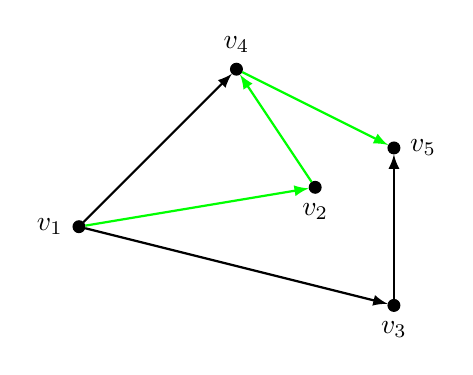
\begin{tikzpicture}

      \tikzset{enclosed/.style={draw, circle, inner sep=0pt, minimum size=.15cm, fill=black}}
%% Vertices
      	\node[enclosed, label={left: $v_1$}] (v1) at (0,2) {};
      	\node[enclosed, label={below: $v_2$}] (v2) at (3,2.5) {};
    		\node[enclosed, label={below: $v_3$}] (v3) at (4,1) {};
  	    \node[enclosed, label={above: $v_4$}] (v4) at (2,4) {};
     	\node[enclosed, label={right: $v_5$}] (v5) at (4,3) {};
%Edges
		\path [->, >=latex, thick, green](v1) edge node[midway, sloped, above] {} (v2);
		\path [->, >=latex, thick](v1) edge node[midway, sloped, above] {} (v3);
		\path [->, >=latex, thick](v1) edge node[midway, above] {} (v4);
		\path [->, >=latex, thick, green](v2) edge node[near end, sloped, below] {} (v4);
		\path [->, >=latex, thick](v3) edge node[midway, below] {} (v5);
		\path [->, >=latex, thick, green](v4) edge node[near end, sloped, above] {} (v5);

	\end{tikzpicture}
	\caption{Eksempel på en orienteret simpel graf og en vej fra $v_{0}$ til $v_{4}$}
	\label{fig.vaegtetopg}
\end{figure}

Da vægtede grafer har en numerisk vægt på hver kant, kan man således beregne \emph{distancen} fra en knude til en anden i grafen. Distancen fra en knude til en anden kan defineres således:

\begin{defn}[Distance]
Lad $m\in \N $, $G=(V,E,w)$ være en vilkårlig graf og $P$ en vilkårlig, simpel vej i grafen således $P=(v_{1},v_{2},\dotsc,v_{m})$. Lad $e_{v_i,v_{i+1}}$ være en kant, som er incident med $v_i$ og $v_{i+1}$ og $i = 1, 2, \dotsc, m$, da kan distancen beskrives som
	\begin{equation}
	\mathrm{dist}(P)=\sum_{i=1}^{m}w(e_{v_i,v_{i+1}}).
	\end{equation}  
\end{defn}

Man kan således bruge følgende definitioner af \emph{korteste vej} og \emph{længste vej} i en vægtet graf:


\begin{defn} [Korteste vej i vægtet graf]\label{defn:min.vej}
Lad $G=(V,E,w)$ være en vilkårlig, vægtet graf. Da er distancen af den korteste simple vej, fra en knude, $v_1$, til en anden knude, $v_m$, defineret som
	\begin{equation}
		\alpha(v_1,v_m)=\arg \min_{P \in \pazocal{P}}
		\textrm{dist}(P),
	\end{equation}
	hvor $\pazocal{P}$ er mængden af alle simple veje fra $v_1$ til $v_m$.
\end{defn}

På samme vis defineres længste vej:

\begin{defn} [Længste vej i en vægtet graf]
	Lad $G=(V,E,w)$ være en vilkårlig, vægtet graf. Da er distancen af den længste simple vej, fra en knude, $v_1$, til en anden knude, $v_m$, defineret som
	\begin{equation}
		\beta(v_1,v_m)=\arg \max_{P \in \pazocal{P}}
		\textrm{dist}(P),
	\end{equation}
	hvor $\pazocal{P}$ er mængden af alle simple veje fra $v_1$ til $v_m$.
\end{defn}

\begin{exmp}
Betragt \autoref{fig.vaegtetopg} \\
\begin{figure}[H]
\centering
	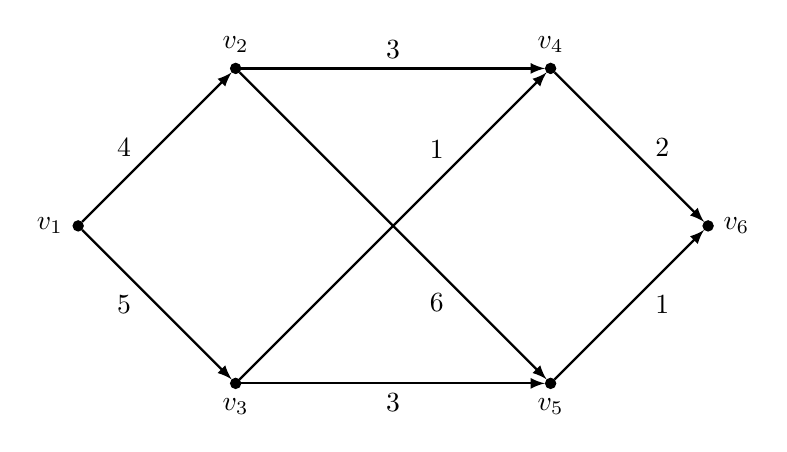
\begin{tikzpicture}

      \tikzset{enclosed/.style={draw, circle, inner sep=0pt, minimum size=.13cm, fill=black}}
%% Vertices
      	\node[enclosed, label={left: $v_1$}] (v1) at (0,2) {};
      	\node[enclosed, label={above: $v_2$}] (v2) at (2,4) {};
    	\node[enclosed, label={below: $v_3$}] (v3) at (2,0) {};
  	    \node[enclosed, label={above: $v_4$}] (v4) at (6,4) {};
     	\node[enclosed, label={below: $v_5$}] (v5) at (6,0) {};
     	\node[enclosed, label={right: $v_6$}] (v6) at (8,2) {};
%Edges
		\path [->, > = latex, thick] (v1) edge node[midway, left=2mm] {4} (v2);
		\path [->, > = latex, thick] (v1) edge node[midway, left=2mm] {$ 5 $} (v3);
		\path [->, > = latex, thick] (v2) edge node[midway, above] {$ 3 $} (v4);
		\path [->, > = latex, thick] (v2) edge node[near end, left=2mm] {$ 6 $} (v5);
		\path [->, > = latex, thick] (v3) edge node[midway, below] {$ 3 $} (v5);
		\path [->, > = latex, thick] (v3) edge node[near end, left=2mm] {$ 1 $} (v4);
		\path [->, > = latex, thick] (v4) edge node[midway, right=2mm] {$ 2 $} (v6);
		\path [->, > = latex, thick] (v5) edge node[midway, right=2mm] {$ 1 $} (v6);

	\end{tikzpicture}
	\caption{Orienteret, simpel og vægtet graf.}
	\label{fig.vaegtetopg}
\end{figure}


På figuren ses en graf med vægtede kanter. Vi er interesserede i at finde den korteste vej fra $v_1$ til $v_6$. For at finde den korteste vej, kigger vi på alle de mulige veje fra $v_1$ til $v_6$.
Følgende veje ses:
\begin{align}
\begin{split}
	P_1=&(v_1,v_2,v_4,v_6)\\
	P_2=&(v_1,v_2,v_5,v_6)\\
	P_3=&(v_1,v_3,v_5,v_6)\\
	P_4=&(v_1,v_3,v_4,v_6)
\end{split}
\end{align}
Man kan nu beregne distancen af de fire veje, ved at tage summen af de kanter, vejen følger. Man får derved:
\begin{align}
\begin{split}
	P_1=&4+3+2=9\\
	P_2=&4+6+1=11\\
	P_3=&5+3+1=9\\
	P_4=&5+1+2=8
\end{split}
\end{align}
Det ses, at den korteste vej fra $v_1$ til $v_6$ er $P_4$. 
Det er sådan, man kan finde korteste vej i en vægtet graf. Denne metode kaldes \emph{brute force}. Metoden kan blive meget tidskrævende ved mere komplekse grafer. I disse tilfælde vil man bruge alternative, bedre algoritmer til at løse problemet. Dette vil vi komme ind på senere i \autoref{kap.algo}.
\end{exmp}

I forhold til korteste vej-problemer er længste vej-problemer betydeligt sværere. For at vise dette betragter vi nu \autoref{fig:laengste.vej}.
\begin{figure}[H]
\centering
	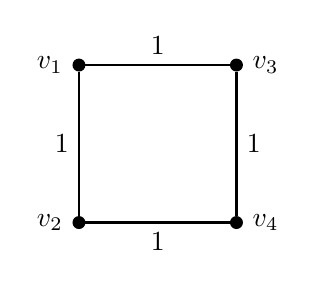
\begin{tikzpicture}
      \tikzset{enclosed/.style={draw, circle, inner sep=0pt, minimum size=.15cm, fill=black}}
%% Vertices
	%ikke orienteret
      	\node[enclosed, label={left, above: $v_1$}] (v1) at (0,2) {};
     	\node[enclosed, label={left, below: $v_2$}] (v2) at (0,0) {};
     	\node[enclosed, label={right, above: $v_3$}] (v3) at (2,2) {};
     	\node[enclosed, label={right, below: $v_4$}] (v4) at (2,0) {};    	
%Edges
	%Ikke orientered
		\path [thick] (v1) edge node[midway, left] {1} (v2);
		\path [thick] (v1) edge node[midway, above] {1} (v3);
		\path [thick] (v2) edge node[midway, below] {1} (v4);
		\path [thick] (v3) edge node[midway, right] {1} (v4);

\end{tikzpicture}
	\caption{Simpel vægtet graf.}
	\label{fig:laengste.vej}
\end{figure}
Vi kan se, at den korteste vej fra $v_1$ til $v_4$ går gennem knuden $v_3$. Vi har dermed også fundet den korteste vej fra $v_1$ til $v_3$.
Hvis vi nu ser på den længste vej fra $v_1$ til $v_4$, går den også igennem $v_3$. I modsætning til korteste vej er den længste vej fra $v_1$ til $v_3$ ikke fundet, da denne går gennem $v_2$ og $v_4$. Derfor er det meget svært at arbejde med længste vej-problemer.
Hvis man til gengæld arbejder med en orienteret acyklisk graf, har man ikke samme problem med at finde længste vej. Dog er det stadig nemmere at finde korteste vej, idet algoritmer til at finde denne er bedre optimeret.
